\documentclass[12pt]{article}
\usepackage[top=1in, bottom=1in, left=.75in, right=.75in]{geometry}
\usepackage{amsmath}
\usepackage{fancyhdr}
\usepackage{graphicx, xcolor}
\usepackage{txfonts}
\usepackage{multicol,coordsys,pgfplots}
\usepackage[scaled=0.86]{helvet}
\renewcommand{\emph}[1]{\textsf{\textbf{#1}}}
\usepackage{anyfontsize}
% \usepackage{times}
% \usepackage[lf]{MinionPro}
\usepackage{tikz,pgfplots}
%\def\degC{{}^\circ{\rm C}}
\def\ra{\rightarrow}
\usetikzlibrary{calc,arrows.meta}
\pgfplotsset{compat = newest}
\newcommand{\blank}[1]{\rule{#1}{0.75pt}}

\pgfplotsset{my style/.append style={axis x line=middle, axis y line=
middle, xlabel={$x$}, ylabel={$y$}}}

%axis equal

%yticklabels={,,} , xticklabels={,,}

% \setmainfont{Times}
% \def\sansfont{Lucida Grande Bold}
\parindent 0pt
\parskip 4pt
\pagestyle{fancy}
\fancyfoot[C]{\emph{\thepage}}
\fancyhead[L]{\ifnum \value{page} > 1\relax\emph{Math 251: Midterm 1}\fi}
\fancyhead[R]{\ifnum \value{page} > 1\relax\emph{Spring 2023}\fi}
\headheight 15pt
\renewcommand{\headrulewidth}{0pt}
\renewcommand{\footrulewidth}{0pt}
\let\ds\displaystyle
\def\continued{{\emph {Continued....}}}
\def\continuing{{\emph {Problem \arabic{probcount} continued....}}\par\vskip 4pt}


\newcounter{probcount}
\newcounter{subprobcount}
\newcommand{\thesubproblem}{\emph{\alph{subprobcount}.}}
\def\problem#1{\setcounter{subprobcount}{0}%
\addtocounter{probcount}{1}{\emph{\arabic{probcount}.\hskip 1em(#1)}}\par}
\def\subproblem#1{\par\hangindent=1em\hangafter=0{%
\addtocounter{subprobcount}{1}\thesubproblem\emph{#1}\hskip 1em}}
\def\probskip{\vskip 10pt}
\def\medprobskip{\vskip 2in}
\def\subprobskip{\vskip 45pt}
\def\bigprobskip{\vskip 4in}

\begin{document}
{\emph{\fontsize{26}{28}\selectfont Spring 2023 \hfill
{\fontsize{32}{36}\selectfont Midterm 2}
\hfill Math F251}}
\vskip 2cm
\strut\vtop{\halign{\emph#\hskip 0.5em\hfil&#\hbox to 2in{\hrulefill}\cr
\emph{\fontsize{18}{22}\selectfont Name:}&\cr
\noalign{\vskip 10pt}
%\emph{\fontsize{18}{22}\selectfont Student Id:}&\cr
%\noalign{\vskip 10pt}
%\emph{\fontsize{18}{22}\selectfont Calculator Model:}&\cr
}}
%\hfill
%\vtop{\halign{\emph{\fontsize{18}{22}\selectfont #}\hfil& \emph{\fontsize{18}{22}\selectfont\hskip 0.5ex $\square$ #}\hfil\cr
%Section: & 001 (Jill Faudree)\cr
%\noalign{\vskip 4pt}
%         & 002 (Ryan Bridges)\cr
%\noalign{\vskip 4pt}
%         & 005 (Leah Berman)\cr}}
%
\vfill
{\fontsize{18}{22}\selectfont\emph{Rules:}}

You have 90 minutes to complete the exam. 

Partial credit will be awarded, but you must show your work.

You may have a single handwritten $3 \times 5$ notecard.

Calculators are not allowed. 


Place a box around your  \fbox{FINAL ANSWER} to each question where appropriate.

%If you need extra space, you can use the back sides of the pages.
%Please make it obvious  when you have done so.

Turn off anything that might go beep during the exam.

Good luck!
\vfill
\def\emptybox{\hbox to 2em{\vrule height 16pt depth 8pt width 0pt\hfil}}
\def\tline{\noalign{\hrule}}
\centerline{\vbox{\offinterlineskip
{
\bf\sf\fontsize{18pt}{22pt}\selectfont
\hrule
\halign{
\vrule#&\strut\quad\hfil#\hfil\quad&\vrule#&\quad\hfil#\hfil\quad
&\vrule#&\quad\hfil#\hfil\quad&\vrule#\cr
height 3pt&\omit&&\omit&&\omit&\cr
&Problem&&Possible&&Score&\cr\tline
height 3pt&\omit&&\omit&&\omit&\cr
&1&&12&&\emptybox&\cr\tline
&2&&10&&\emptybox&\cr\tline
&3&&10&&\emptybox&\cr\tline
&4&&14&&\emptybox&\cr\tline
&5&&16&&\emptybox&\cr\tline
&6&&10&&\emptybox&\cr\tline
&7&&8&&\emptybox&\cr\tline
&8&&8&&\emptybox&\cr\tline
&9&&12&&\emptybox&\cr\tline
&Extra Credit&&5&&\emptybox&\cr\tline
&Total&&100&&\emptybox&\cr
}\hrule}}}

\newpage
\begin{enumerate}
%%%%
%% antiderivatives
\item (12 points) Evaluate the indefinite integrals below. 
	\begin{enumerate}
	\item $\displaystyle \int \left( 8x^{2/3} +\sec(x)\tan(x) \right) \: dx$
	\vfill
	\item $\displaystyle \int \left( e^x +2 \right) \: dx$
	\vfill
	\item $\displaystyle \int \frac{1+x^3}{x^2} \: dx$
	\vfill
	\end{enumerate}
	
	%%%%
%% Linear Approximation
\item (10 points)
\begin{enumerate}
\item Find the linear approximation, $L(x),$ to $f(x)=\sqrt{x}$ at $a=25.$
\vspace{1.5in}
\item Use your answer in part $a$ to estimate $\sqrt{23}.$ Your answer should be in the form of a simplified fraction or a decimal.
\vspace{1.5in}
\end{enumerate}

\newpage

%%%%
%% Related rate
\item (10 points) If a airplane is flying at a constant speed of 100 miles per hour and is climbing at a an angle of 30 degrees, at what rate is its altitude changing? Your final answer should include units.\\

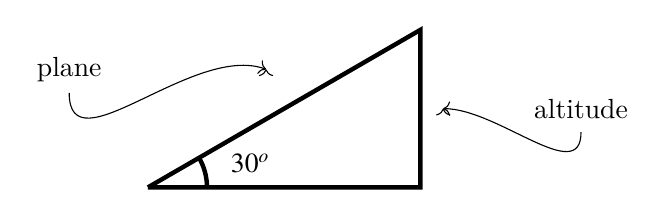
\begin{tikzpicture}[scale=1]
\draw[ultra thick] (0,0)--(3.46,0)--(3.46,2)--(0,0);
\draw[ultra thick] (0:0.75) arc (0:30:0.75);
\node at (1.3,0.3){$30^o$};
\node at (-1,1.5){plane};
\node at (5.5,1){altitude};
\draw[thin,<-] (1.5,1.5) edge [out=160, in=270] (-1,1.2);
\draw[thin,<-] (3.75,1) edge [out=0, in=270] (5.5,0.7);
\end{tikzpicture}

\newpage
%%%%
%% Derivatives and shape of graph
\item (14 points) Let $\displaystyle f(x)=\ln(x^2+2).$ It is a fact that $\displaystyle f'(x)=\frac{2x}{x^2+2}$ and $\displaystyle f''(x)=\frac{-2(x^2-2)}{(x^2+2)^2}.$
\begin{enumerate}
	\item Determine intervals where $f(x)$ is increasing or decreasing.
	\vfill
	\item Identify any local maxima or minima or state that none exist and their location. \\(Your answer should be in the form: ``$f$ has a local maximum/minimum of \underline{\hspace{.3in}} at \underline{\hspace{.3in}}" or \\``$f$ has no local maxima/minima.")
	\vspace{1.5in}
	\item Determine intervals where $f(x)$ is concave up or concave down.
	\vfill
	\item Identify all inflection points or state that none exist.
	\vspace{1in}
	\end{enumerate}
\newpage
%%%%
%% L'Hop Rule and Limits at infinity
\item (16 points) Evaluate the limits below. You must show your work. Indicate an application of L'H\^{o}pital's Rule by putting an $H$ above equal sign.
\begin{enumerate}
	\item $\displaystyle \lim_{x \to 0} \frac{e^x-\cos(x)}{4\tan(x)}$
	\vfill
	\item $\displaystyle \lim_{x \to \infty} \frac{\ln(x)}{x^{1/2}}$
	\vfill
	\item $\displaystyle \lim_{x \to 0^+} \left( 1+ x \right)^{\frac{1}{2x}}$
	\vfill
\end{enumerate}

\newpage



%%%%
%% Optimization
\item (10 points) An open-topped box with a square base has a fixed surface area of $1200 \: \text{in}^2.$ Determine the dimensions of the box with maximum volume. Justify your answer using Calculus.

\newpage


%%%%
%% approximating rectangles
\item (8 points) The function $f(x)=\frac{24}{x+1}$ is graphed below. We want to estimate the area under the curve $f(x)$ on the interval $[0,8]$ using $M_4.$ (That is, we want to use 4 approximating rectangles with midpoints determining height.) 

\begin{multicols}{2}
\begin{enumerate}
\item Sketch the four approximating rectangles on the graph. 

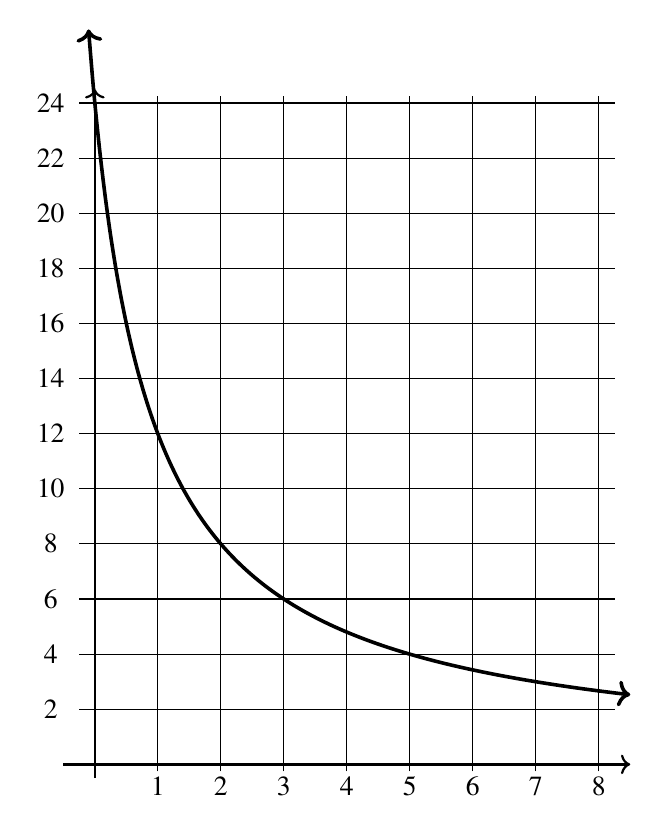
\begin{tikzpicture}[xscale=.8, yscale=0.35]
\draw[thick, ->] (0,-0.5) -- (0,24.5);
\draw[thick, ->] (-0.5,0) -- (8.5,0);
\foreach \j in {1,2,3,4,5,6,7,8}{
	\draw (\j,-0.25) -- (\j, 24.25);
	\node at (\j,-.8){$\j$};
	}
\foreach \j in {2,4,6,8,10,12,14,16,18,20,22,24}{
	\draw (-0.25,\j) -- (8.25,\j);
	\node at (-0.7,\j){$\j$};
	}
\draw[<->,line width=1.3pt,smooth,samples=100,domain=-0.1:8.5] plot(\x,{24/(\x+1)});
\end{tikzpicture}
\columnbreak
\item Do a calculation to estimate the area under the curve using $M_4$ (that is, use 4 approximating rectangles and midpoints) and simplify your answer. \\
\end{enumerate}
\end{multicols}

%%%%
%% definite integral using geometry
\item (8 points) Evaluate the definite integrals below using the graph of $H(x)$ and properties of definite integrals. On the interval $[3,7],$ the graph of $H$ is a semi-circle. Show your work.

\begin{multicols}{2}
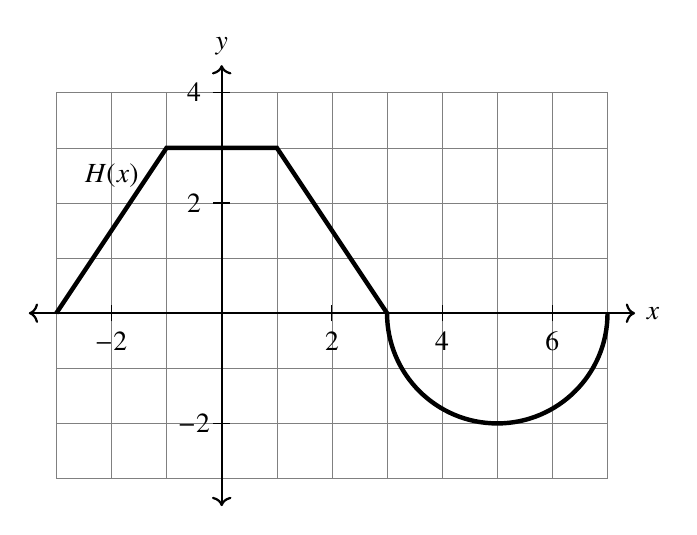
\begin{tikzpicture}[scale=.7]
\draw[help lines] (-3,-3) grid (7, 4);
\draw[<->, thick] (-3.5, 0) -- (7.5, 0) node[right] {$x$};
\draw[<->, thick] (0, -3.5) -- (0,4.5) node[above] {$y$};
\draw[ultra thick] (-3,0) -- (-1,3) -- (1,3) -- (3,0);
\draw[ultra thick] (3,0) arc (180:360:2);
\foreach \j in {-2,2,4,6}{
	\draw (\j,-0.15) -- (\j, 0.15);
	\node at (\j,-.5){$\j$};
	}
\foreach \j in {-2,2,4}{
	\draw (-0.15,\j) -- (0.15,\j);
	\node at (-0.5,\j){$\j$};
	}
\node at (-2,2.5) {$H(x)$};
\end{tikzpicture}

\columnbreak

\begin{enumerate}
\item $\displaystyle{\int_{-3}^7 f(x) \: dx}$
\vfill
\item
$\displaystyle{\int_{0}^3 (4 f(x)+6) \: dx}$

\end{enumerate}
\end{multicols}
\quad

\vspace{1in}

\newpage
%%%%
%% Sketch
\item (12 points) Sketch a graph that satisfies all the criteria in the list below.\\

\begin{multicols}{2}
\begin{itemize}
\item Domain $(-\infty, \infty)$
\item $f(0)=1$
\item $f'(x) < 0$ on $(-\infty, \infty)$
\item $f''(x) < 0$ on $(-\infty, 0)$, $f''(x) > 0$ on $(0,\infty)$
\end{itemize}

\quad

\vspace{.3in}

\quad
 \columnbreak
 
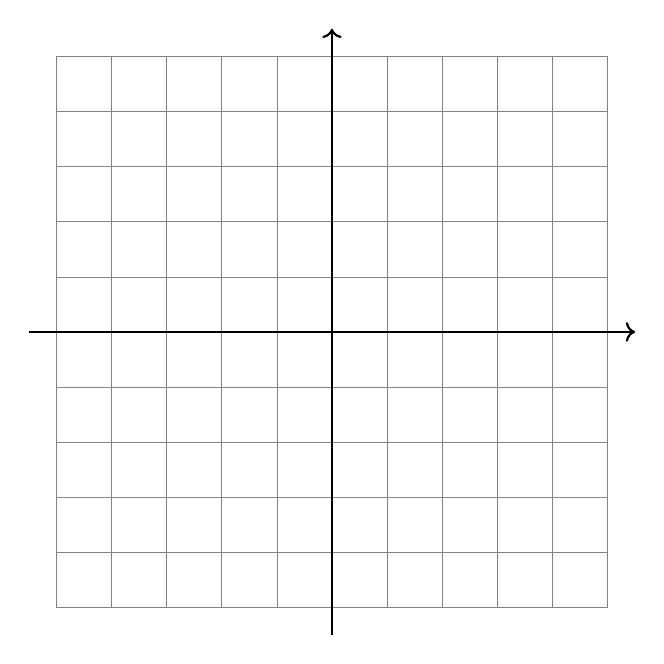
\begin{tikzpicture}[scale=.7]
\draw[help lines] (-5,-5) grid (5,5); 
\draw[thick, ->] (0,-5.5) -- (0,5.5);
\draw[thick, ->] (-5.5,0) -- (5.5,0);
\end{tikzpicture}
\end{multicols}
\end{enumerate}



\textbf{Extra Credit} (5 points) Identify all vertical and horizontal asymptotes of the function $f(x)=\frac{4e^x+1}{7e^x-1}$. Justify your answer using limits.
\vfill

\end{document}

%%%%ENDDOCUMENT


